



In this section, we consider Problem~\ref{prob:det_unary_length} at delay 1 first and then at arity 1. 
Let $\Xi = (\Sigma, R, \delta, \alpha, \sigma, w)$ be a deterministic oritatami system of delay 1. 
For $i \geq 0$ let $C_i$ be the unique elongation of $\sigma$ by $w[1..i]$, that is, foldable by $\Xi$. Hence $C_0 = \sigma$.

\begin{comment}
\begin{figure}
  \begin{center}
    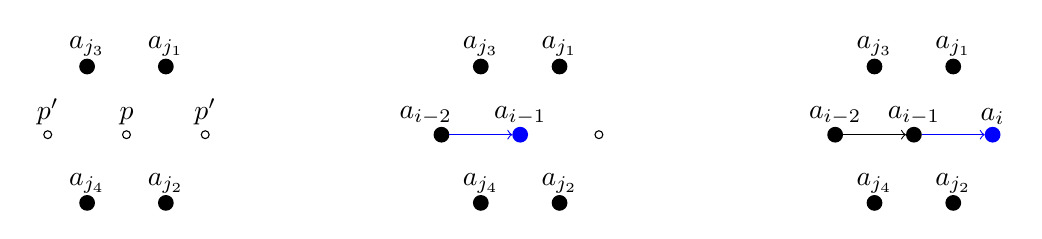
\begin{tikzpicture}
      \draw (0:0) circle [radius=0.05];
      \draw (0:1) circle [radius=0.05];
      \draw (180:1) circle [radius=0.05];
      \node[above] at (0:1) { $p^\prime$ };
      \node[above] at (0:0) { $p$ };
      \node[above] at (180:1) { $p^\prime$ };
      
      \fill (60 : 1) circle [radius=0.1];
      \fill (-60 : 1) circle [radius=0.1];
      \fill (120 : 1) circle [radius=0.1];
      \fill (-120 : 1) circle [radius=0.1];
      \node[above] at (60 :1) { $a_{j_1}$ };
      \node[above] at (-60 :1) { $a_{j_2}$ };
      \node[above] at (120 :1) { $a_{j_3}$ };
      \node[above] at (-120 :1) { $a_{j_4}$ };
      
      \begin{scope}[shift=(0:5)]
        \fill[blue] (0:0) circle [radius=0.1];
        \draw (0:1) circle [radius=0.05];
        \fill (180:1) circle [radius=0.1];
        \node[above] at (180:1.2) { $a_{i-2}$ };
        \node[above] at (0:0) { $a_{i-1}$ };
        \draw[->, blue] (180:0.9) -- (180:0.1);
        
        \fill (60 : 1) circle [radius=0.1];
        \fill (-60 : 1) circle [radius=0.1];
        \fill (120 : 1) circle [radius=0.1];
        \fill (-120 : 1) circle [radius=0.1];
        \node[above] at (60 :1) { $a_{j_1}$ };
        \node[above] at (-60 :1) { $a_{j_2}$ };
        \node[above] at (120 :1) { $a_{j_3}$ };
        \node[above] at (-120 :1) { $a_{j_4}$ };
      \end{scope}
      \begin{scope}[shift=(0:10)]
        \fill (0:0) circle [radius=0.1];
        \fill[blue] (0:1) circle [radius=0.1];
        \fill (180:1) circle [radius=0.1];
        \node[above] at (180:1) { $a_{i-2}$ };
        \node[above] at (0:0) { $a_{i-1}$ };
        \node[above] at (0:1) { $a_i$ };
        \draw[->] (180:0.9) -- (180:0.1);
        \draw[->,blue] (0:0.1) -- (0:0.9);
        
        \fill (60 : 1) circle [radius=0.1];
        \fill (-60 : 1) circle [radius=0.1];
        \fill (120 : 1) circle [radius=0.1];
        \fill (-120 : 1) circle [radius=0.1];
        \node[above] at (60 :1) { $a_{j_1}$ };
        \node[above] at (-60 :1) { $a_{j_2}$ };
        \node[above] at (120 :1) { $a_{j_3}$ };
        \node[above] at (-120 :1) { $a_{j_4}$ };
      \end{scope}
    \end{tikzpicture} 
    \caption{Through a tunnel section}
    \label{TTT_tunnel_intro}
  \end{center}
\end{figure}
\end{comment}

\begin{figure}[tb]
  \begin{center}
    \begin{tabular}{ccc}
      
      \begin{minipage}{0.3\hsize}
        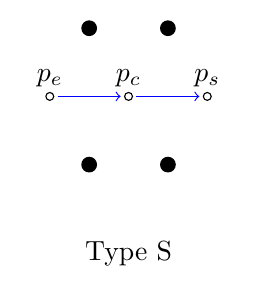
\begin{tikzpicture}
          \begin{scope}[xshift=2cm, yshift=2cm]
          
            \draw[white] (60:1) -- (0:0);
            \draw[white] (-60:1) -- (0:0);
            \draw(0,0) circle [radius=0.05];
            \node[above] at (0,0) {$p_c$};
            \node[above] at (180:1) {$p_e$};
            \node[above] at (0:1) {$p_s$};

            \foreach \theta in {0,180}{
              \draw[transform canvas={shift=(\theta:1)}](0,0) circle [radius=0.05];
            }
            
            \foreach \theta in {60,-60,120,-120}{
              \fill[transform canvas={shift=(\theta:1)}](0,0) circle [radius=0.1];
            }
          \draw[->, blue] (-0.9, 0) -- (-0.1, 0);
          \draw[->, blue] (0.1, 0) -- (0.9, 0);
          \end{scope}
          

          \node at (2,0) {Type S};
        \end{tikzpicture}
      \end{minipage}

      \begin{minipage}{0.3\hsize}
        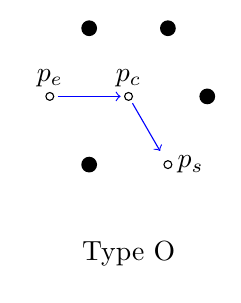
\begin{tikzpicture}

          \begin{scope}[xshift=2cm, yshift=2cm]
          
            \draw[white] (60:1) -- (0:0);
            \draw[white] (-60:1) -- (0:0);
            \draw(0,0) circle [radius=0.05];
            \node[above] at (0,0) {$p_c$};
            \node[above] at (180:1) {$p_e$};
            \node[right] at (-60:1) {$p_s$};

            \foreach \theta in {-60,180}{
              \draw[transform canvas={shift=(\theta:1)}](0,0) circle [radius=0.05];
            }
            
            \foreach \theta in {0,60,120,-120}{
 	            \fill[transform canvas={shift=(\theta:1)}](0,0) circle [radius=0.1];
            }
          \draw[->, blue] (-0.9, 0) -- (-0.1, 0);
          \draw[->, blue] (0,0)++(300:0.1) -- (300:0.8);
          \end{scope}

          \node at (2,0) {Type O};
        \end{tikzpicture}
      \end{minipage}

      \begin{minipage}{0.3\hsize}
        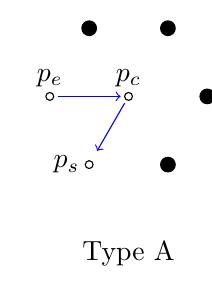
\begin{tikzpicture}

          \begin{scope}[xshift=2cm, yshift=2cm]
            \draw[white] (60:1) -- (0:0);
            \draw[white] (-60:1) -- (0:0);
            \draw(0,0) circle [radius=0.05];
            \node[above] at (0,0) {$p_c$};
            \node[above] at (180:1) {$p_e$};
            \node[left] at (-120:1) {$p_s$};

            \foreach \theta in {-120,180}{
              \draw[transform canvas={shift=(\theta:1)}](0,0) circle [radius=0.05];
            }
            
            \foreach \theta in {0,60,-60,120}{
              \fill[transform canvas={shift=(\theta:1)}](0,0) circle [radius=0.1];
            }
          \draw[->, blue] (-0.9, 0) -- (-0.1, 0);
          \draw[->, blue] (0,0)++(240:0.1) -- (240:0.8);
          \end{scope}

          \node at (2,0) {Type A};
        \end{tikzpicture}
      \end{minipage}
      
    \end{tabular}
    \caption{Tunnel sections of all possible three types: straight (Type S), obtuse turn (Type O), and acute turn (Type A).}
    \label{fig:TTT_tunnel}
  \end{center}
\end{figure}

At delay 1, a bead cannot collaborate with its successors in order to stabilize itself. 
In fact, there are just two ways for a bead to get stabilized at delay 1 (or the bead has no place to be stabilized around so that the system halts), as observed in \cite{DHOPRSST2018}. 
One is to be bound to another bead and the other is through a 1-in-1-out structure called the tunnel section. 
See Fig.~\ref{fig:TTT_tunnel}. 
A \textit{tunnel section} consists of one free point $p_c$ and four beads that occupy four neighbors of $p_c$. 
In order for an oritatami system to stabilize the bead $w[i]$ at the central point $p_c$, its predecessor $w[i-1]$ must be put at one of the two free neighbors of $p$. 
Thus, at the stabilization of $w[i]$, only one neighbor of $p$ is left free so that the successor $w[i+1]$ is to be stabilized there, even without being bound. 
In this case, the point $p_e$ where $w[i-1]$ is stabilized is considered to be an \textit{entrance of the tunnel section} and the point $p_s$ where $w[i+1]$ is stabilized is considered as its \textit{exit}. 
A \textit{tunnel} is a maximal set of tunnel sections whose central points form a path. 

The behavior of an oritatami system at delay 1 can be described by a sequence of $S$ of $b$ (bound), $t_s$ (straight tunnel section), $t_o$ (obtuse-turn tunnel section), and $t_a$ (acute-turn tunnel section); priority is given to tunnel, that is, $S[i]$ is $t_s$ (resp.~$t_o$, $t_a$) if the $i$-th bead of the system is stabilized not only by being bonded but also through a straight (resp. obtuse-turn, acute-turn) tunnel section. 
Let us introduce $t$ as a wildcard for $t_s$, $t_o$, and $t_a$. 
We also let $S$ take the value $\blacksquare$ for halt (due to the lack of free neighbors). 

%If a bead is stabilized through a tunnel section, then it can provide some bonds. Let us consider bonds of $C_i$. $C_i$ is represented $C = (W,P,H)$ where $|W| = i + n$ $C_i$ contains $\alpha \cdot (i + n) - 2|H|$ bonds because $C_i$ consists of $i + n$ beads and a bead has just $\alpha$ bonds and then $2 |H|$ of the those bonds are already used. However, even if a bead has an available bond, $w[j]$ $(j > i)$ might not be able to use this bond because the bond has possibility that it is blocked by transcripts $w[i+1..j-1]$. Number of $binding\ capabilities$ does not contain that case so that it is at most $\alpha \cdot (i + n) - 2|H|$.

\begin{figure}[tb]
\centering
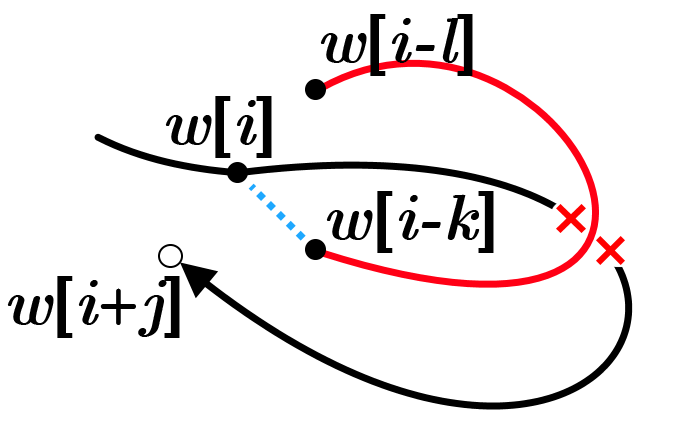
\includegraphics[width=0.5\linewidth]{Fig/jordan_curve.png}
\caption{A tunnel divides the world into two. 
%Getting through the tunnel leads us to another world. 
}
\label{fig:Jordan}
\end{figure}

%We say that point $p$ is reachable from a conformation $C$ if there exists a directed path $P^\prime$ from the last point of $C$ that does not cross the path of $C$. 
We say that a neighbor of a point $p$ is \textit{reachable} from a conformation $C$ if there exists an elongation of $C$ in which a bead occupies the neighbor and it binds with a bead at $p$. 
For example, in Fig.~\ref{fig:Jordan}, the transcript $w$ is about to step into a tunnel. 
The wall beads $w[i-\ell]$ and $w[i-k]$ are both older than the bead at the entrance, $w[i]$. 
Even if $w[i]$ leaves a free neighbor, the neighbor is not reachable because the the path of a conformation must be non-self-intersecting, and its subpath between these two wall beads divides the plane into two regions, one of which includes the entrance of the tunnel and the other of which includes the exit (Jordan curve theorem \cite{Hales2007}). 
Taking this reachability into account, we define the \textit{binding capability} of a conformation as the number of free bonds of its beads available geometrically for elongations of $C$.
It is defined formally as follows: 

\begin{definition}[Binding Capability]
Let $\alpha$ be an arity and $C = (P,w,H)$ be a conformation of arity at most $\alpha$.
Let $H_k = H \cap \{ (i,j) \mid \mbox{$i=k$ or $j=k$} \}$. 
Moreover, let $R_k$ be a set of neighbors of the point $P[k]$ that are free and reachable from $C$.
The binding capability of $C$ at arity $\alpha$, denoted by $\#bc_\alpha(C)$, is defined by $\sum^{|w|}_{k=1} \min \{\alpha-|H_k|, |R_k|\}$.
The subscript $\alpha$ is omitted whenever it is clear from context. 
\end{definition}
%
Observe one almost-trivial but important fact that a bead inside a tunnel does not increase the binding capability. 
This is because for such a bead $w[k]$, $|R_k| = 0$. 

We now prove that in ``almost all'' tunnels is a troll domiciled and robs the transcript of binding capability (the original story is from \cite{Pratchett1992}). 
Originally, we tried to find a troll in every tunnel but failed; a troll seems to dislike the very first bead $w[1]$, or its property that only $\alpha$+1 beads around may take all hands of $w[1]$ thanks to the absence of its predecessor; any other bead must be surrounded by at least $\alpha+2$ beads in order to be free from free hand because a bead cannot bind with its predecessor or successor. 
We call a bead \textit{singular} if it is surrounded by only $\alpha+1$ beads but forms $\alpha$ bonds. 
No bead but $w[1]$ can be singular because of their predecessor and successor. 
A tunnel is \textit{singular} if its entrance or exit is next to $w[1]$ that is singular. 
There can be at most 3 tunnels around one bead so that no more than 3 tunnels can be singular. 
A singular tunnel will be denoted with the superscript $\times$ like $t_s^\times$ or $t^\times$. 
In contrast, the notation without $\times$ such as $t_s$ and $t$ shall imply their non-singularity. 

